%%% Ne pas modifier jusqu'à la ligne 25
\documentclass[a4paper,12pt]{book}
\usepackage[utf8]{inputenc}
\usepackage[french]{babel}
%%\usepackage{CJK}
\usepackage{yhmath}
\usepackage[left=2cm,right=2cm,top=3cm,bottom=2cm, headheight=1.5cm,headsep=1.5cm]{geometry}
%%\usepackage{CJKutf8}
\usepackage{amsfonts}
\usepackage{mathrsfs}
\usepackage{amsmath,amsfonts,amssymb,dsfont}
\usepackage{graphicx}
\usepackage{subfigure}
\usepackage{enumitem}		%\enumerate-resume
\usepackage[colorlinks=true,unicode={true},hyperindex=false, linkcolor=blue, urlcolor=blue]{hyperref}
\newcommand{\myref}[1]{\ref{#1} page \pageref{#1}}

\addto\captionsfrench{\def\tablename{Tableau}}  %légendes des tableaux
\renewcommand\thesection{\Roman{section}~-~} 
\renewcommand\thesubsection{\Roman{section}.\Alph{subsection}~-~} 
\renewcommand\thesubsubsection{\Roman{section}.\Alph{subsection}.\arabic{subsubsection}~-~} 

\newcommand{\conclusion}[1]{\newline \centerline{\fbox{#1}}}

\setcounter{secnumdepth}{3}
\parindent=0pt

\usepackage{fancyhdr}
\pagestyle{fancy}

\lhead{SJTU-ParisTech} 
%%%%%%%%%%%%%%%%%%%%%%%%%%%%%%%%%%
\chead{DM}
\rhead{Daniel 518261910024}

\begin{document}
\renewcommand{\labelitemi}{$\blacktriangleright$}
\renewcommand{\labelitemii}{$\bullet$}


\section{TD 1-1}
\begin{figure}[h]
    \begin{center}
    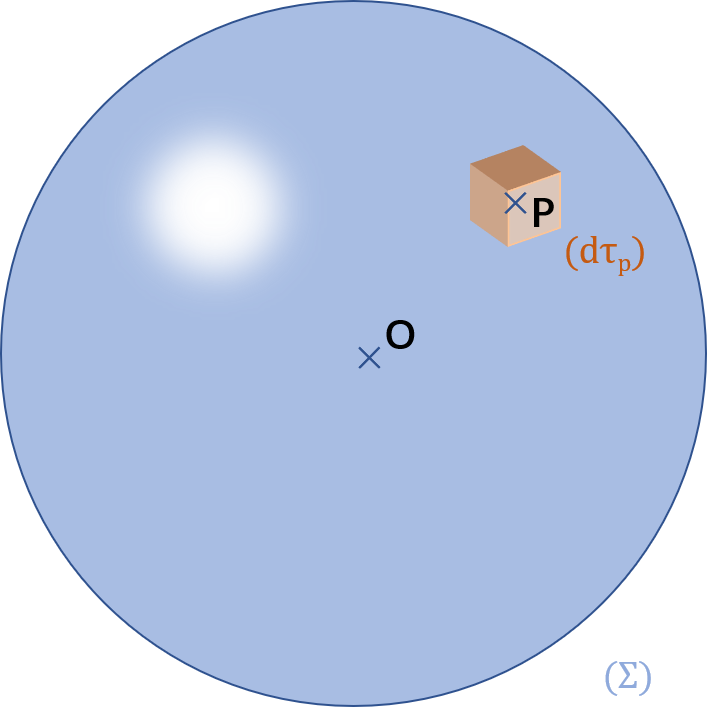
\includegraphics[scale=0.6]{elec11.png}
    \end{center}
    \caption{le système étudiée}
\end{figure}
Le système $(\Sigma)$ étudiée: Le noyau d'un atome d'hydrogène

On a la charge élémentaire $\delta Q=\rho(P,t)\,d\tau_P$, avec $\rho(P,t)$ la densité volumique de charge.
Pour une répartie uniformément et supposant que la charge est indépendant du temps, on a $\rho(P,t)=\rho$

Dans le modèle d'une distribution de charge continue, on a 
$$
Q=e=\iiint_{P \in (\Sigma)} \rho\,d\tau_P=\rho\iiint_{P \in (\Sigma)}d\tau_P=\frac{4}{3}\pi R^3\rho
$$
On a donc $\boxed{\rho=\frac{3Q}{4\pi R^3}}$

A.N. $\boxed{\rho=\frac{3\times 1,602\times10^{-19}}{4 \times 3.14\times (1\times 10^{-15})^2}=4\times 10^{25}\,C\cdot m^{-3}}$


\section{TD 2-1}
\begin{figure}[h]
    \begin{center}
    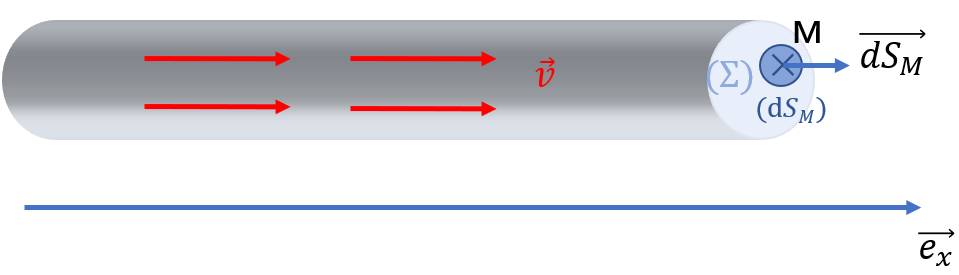
\includegraphics[scale=0.6]{elec12.png}
    \end{center}
    \caption{le système étudiée}
\end{figure}
Supposons que la vitesse moyenne $\vec{v}$ est indépendant du temps, on a donc le vecteur densité volumique 
$$
\vec{j}(M,t)=nq\vec{v}=nqv\vec{e}_x
$$
avec $n$ la densité volumique, $q=-e$ la charge du chaque atome de cuivre. 
On a donc 
$$
I=\left|\iint_{M \in (\Sigma)}\vec{j}(M,t)\,\vec{dS_M}\right|=\left|nqv\iint_{M \in (\Sigma)}\vec{dS_M}\right|=\left|nqv\pi a^2\right|
$$ 
Par définition, $n=\frac{dN}{dV}$ le nombre d'atomes molaire, donc 
$$
n=\frac{dN}{dV}=\frac{\frac{dm}{M}N_A}{dV}=\frac{\mu N_A}{M}
$$
Donc 
$$
I=\frac{\mu N_A}{M}ev\pi a^2
$$
Finalement, on a 
$$
\boxed{v=\frac{IM}{\mu N_Ae\pi a^2}}
$$
A.N. $\boxed{v=\frac{10\times 63.55}{8.960*10^6\times 6.02*10^23\times 1.6*10^{-19}\times 3.14\times (1,0*10^{-3})^2}=2.3*10^{-4}\,m\cdot s^{-1}}$

\end{document}